\chapter{Physics-Informed LSTM Network For Velocity Prediction of Fluid Flow Simulations}
\section{The Importance of Fluid Flow Velocity Prediction}
In fluid flow velocity prediction you model a system that describes some physical geometry and specific fluids with some initial boundary conditions and predict how these fluids will flow and interact in the system and what the fluid velocities will be at every point in the system after a certain amount of time has passed given the initial boundary conditions. This problem is important in mechanical engineering as the mechanical designs of airplane wings, turbines, and other important machinery are based on how they will interact with the flow of air, water, and other particles in the atmosphere or environment where they are used.

\begin{figure}[H] \centering
    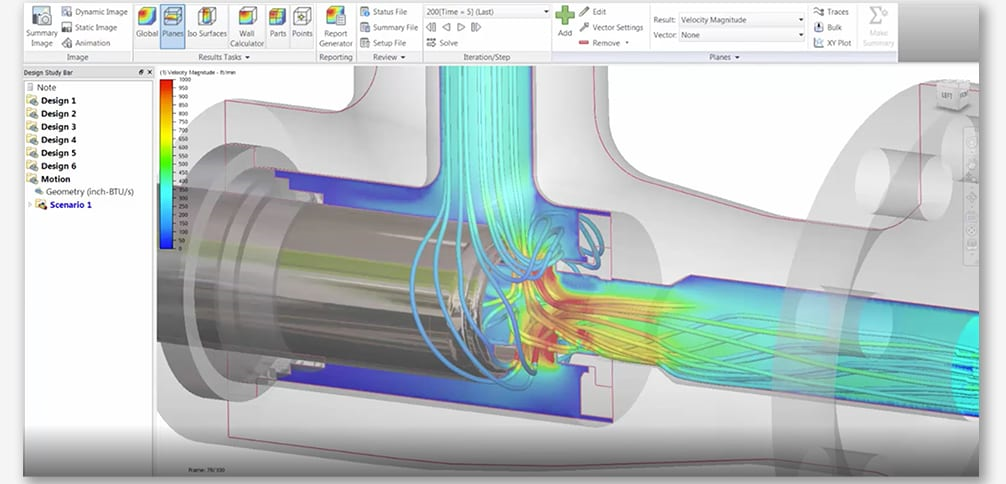
\includegraphics[width=\linewidth]{figures/cfd_engine.png}
    \caption{An example of a Computational Fluid Dynamics (CFD) simulation predicting the fluid flow velocities in an engine.}
    \label{fig:cfd_engine}
\end{figure}


\section{Long Short-Term Memory Networks (LSTMs) For Time Series Data}
\begin{figure}[H] \centering
    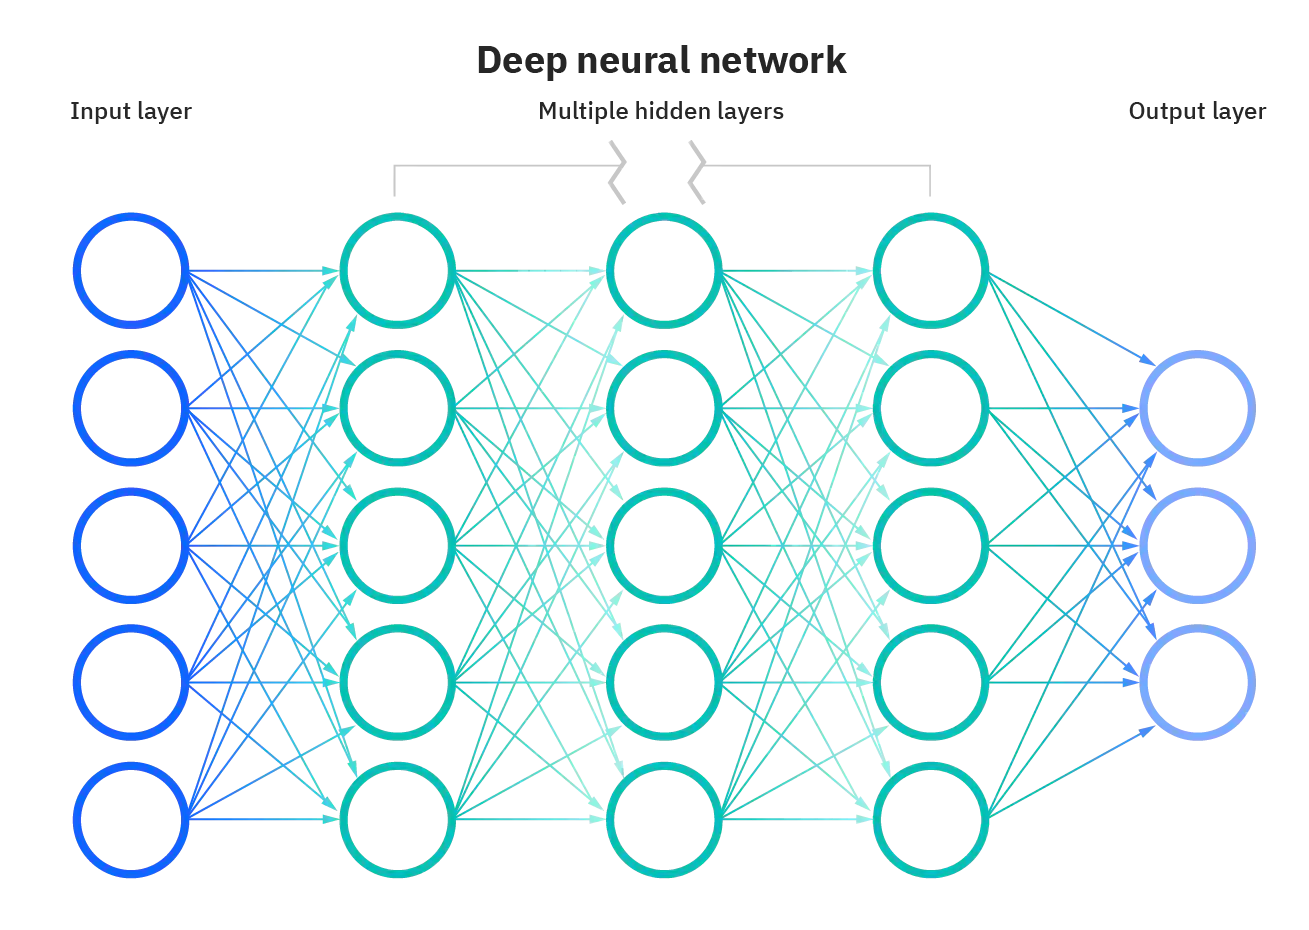
\includegraphics[width=0.4\linewidth]{figures/neural_network.png}
    \rulesep
    % https://www.asimovinstitute.org/neural-network-zoo/
    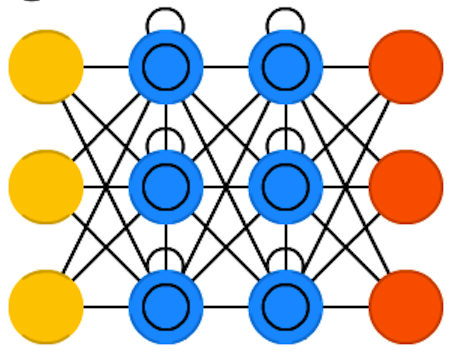
\includegraphics[width=0.4\linewidth]{figures/lstm.png}
    \caption{A regular 3-layer dense neural network on the left, an LSTM on the right. On the LSTM the blue dots with circles are the specialized LSTM cells, and note how self-connections from RNNs are present in LSTMs as well.}
    \label{fig:neural_network_and_lstm}
\end{figure}

Long Short-Term Memory Networks (LSTMs) \cite{LSTM} are neural network models designed to learn long term dependencies in sequential datasets and are a variation of the Recurrent Neural Network (RNN). LSTMs selectively pick and store short-term information that might be useful to know for later using a unique cell structure that includes an input, forget, and output gate. These gates determine what past information to forget and what new information to keep track of and it is through this mechanism of storing short memories for a long period of time where ``long'' short-term memory derives the name from.

% https://towardsdatascience.com/lstm-recurrent-neural-networks-how-to-teach-a-network-to-remember-the-past-55e54c2ff22e
\begin{figure}[H] \centering
    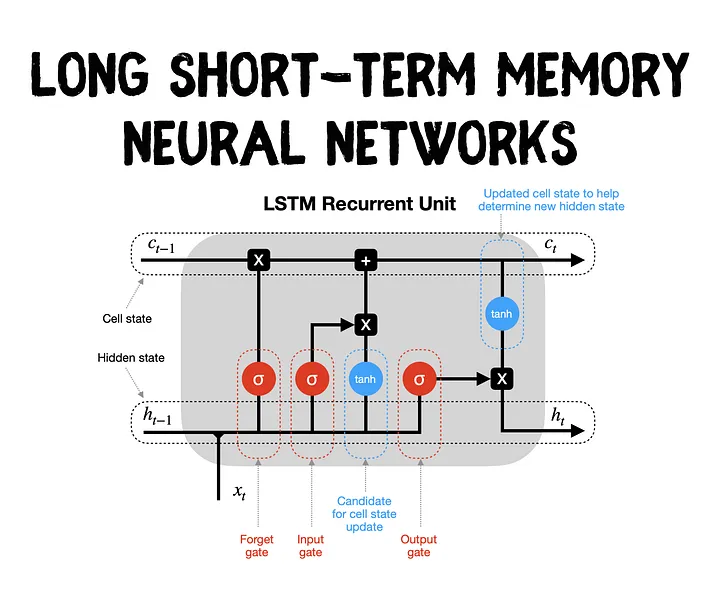
\includegraphics[width=0.8\linewidth]{figures/lstm_unit.png}
    \caption{An LSTM cell or unit showing all the gates and operations.}
    \label{fig:lstm_cell}
\end{figure}

\section{Adding Physics to LSTMs}
I began to tackle the problem of fluid flow predictions by creating a new neural network architecture based on a combination of Physics-Informed Neural Networks (PINNs) and Long-Short Term Memory Networks (LSTMs) \cite{Perez2022}. Specifically, we created a two-branch network architecture that takes as inputs the measurements taken from a Computational Fluid Dynamic (CFD) simulation and predicts what the velocity components (in 2D) will be for a given timestep.

\subsection{Fluid Flow Velocity Data From Simulations}
The data was generated using Ansys by creating a simulation in which we modeled a water-braking scoop mechanism in 2D space, constraining the domain of the model to a 2.2 meter by 4 meter box and running the simulation with different inlet velocity profiles. The simulation geometry, mesh, and boundary conditions can be seen in Figures \ref{fig:cfd_geometry}, \ref{fig:cfd_mesh}, and \ref{fig:cfd_boundary_conditions} in the Introduction section.

The following figures demonstrate the simulation results for different boundary conditions at specific times in the simulation. For the figures with two pictures, the left picture represents the pressure and velocity contours and the right picture the velocity and water volume fraction.

\begin{figure}[H] \label{fig:fluid_sim1} \centering
    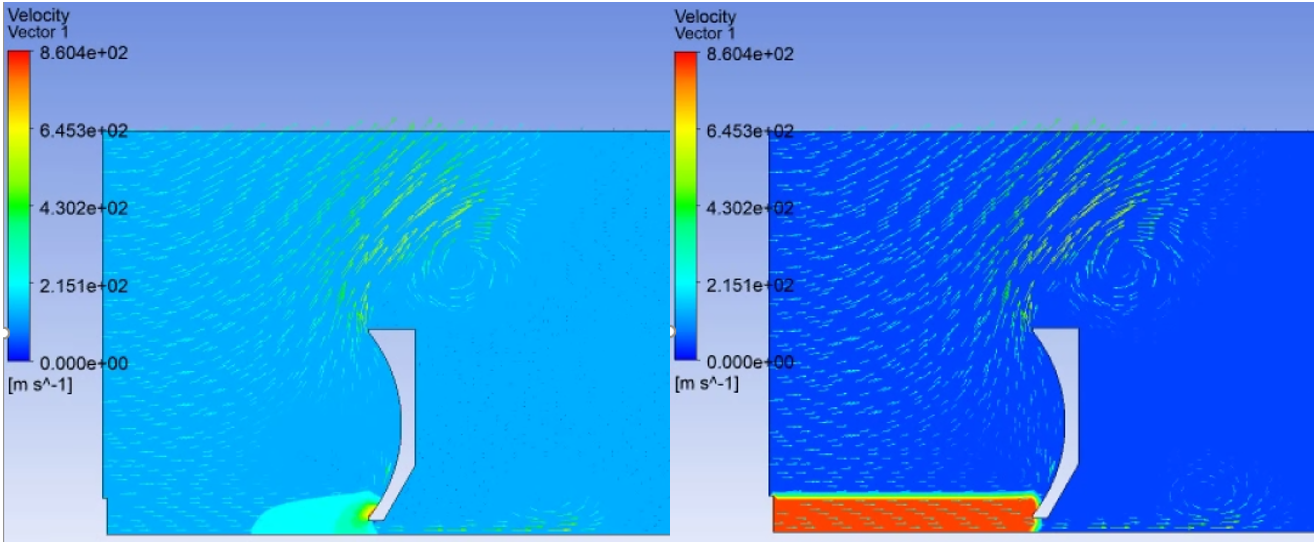
\includegraphics[width=\linewidth]{figures/fluid_sim1.png}
    \caption{Velocity Inlet = $250 m/s$, Time = $0.011sec$}
\end{figure}

\begin{figure}[H] \label{fig:fluid_sim3} \centering
    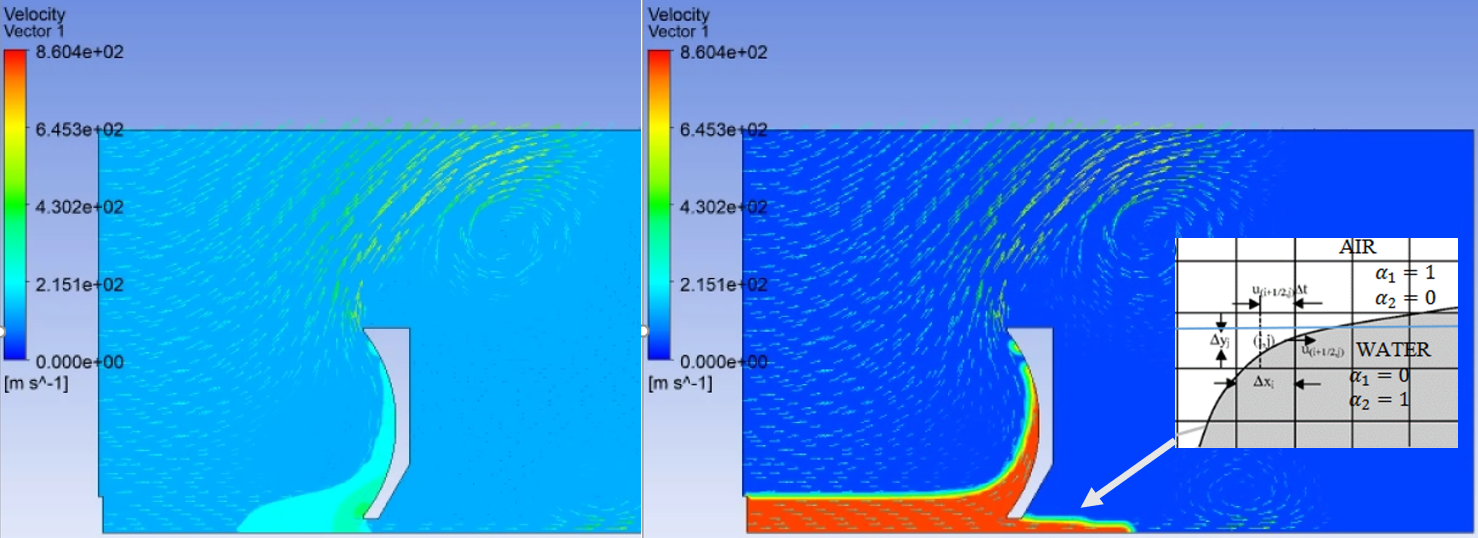
\includegraphics[width=\linewidth]{figures/fluid_sim3.png}
    \caption{Velocity Inlet = $250 m/s$, Time = $0.016sec$.}
\end{figure}

\begin{figure}[H] \label{fig:fluid_sim2} \centering
    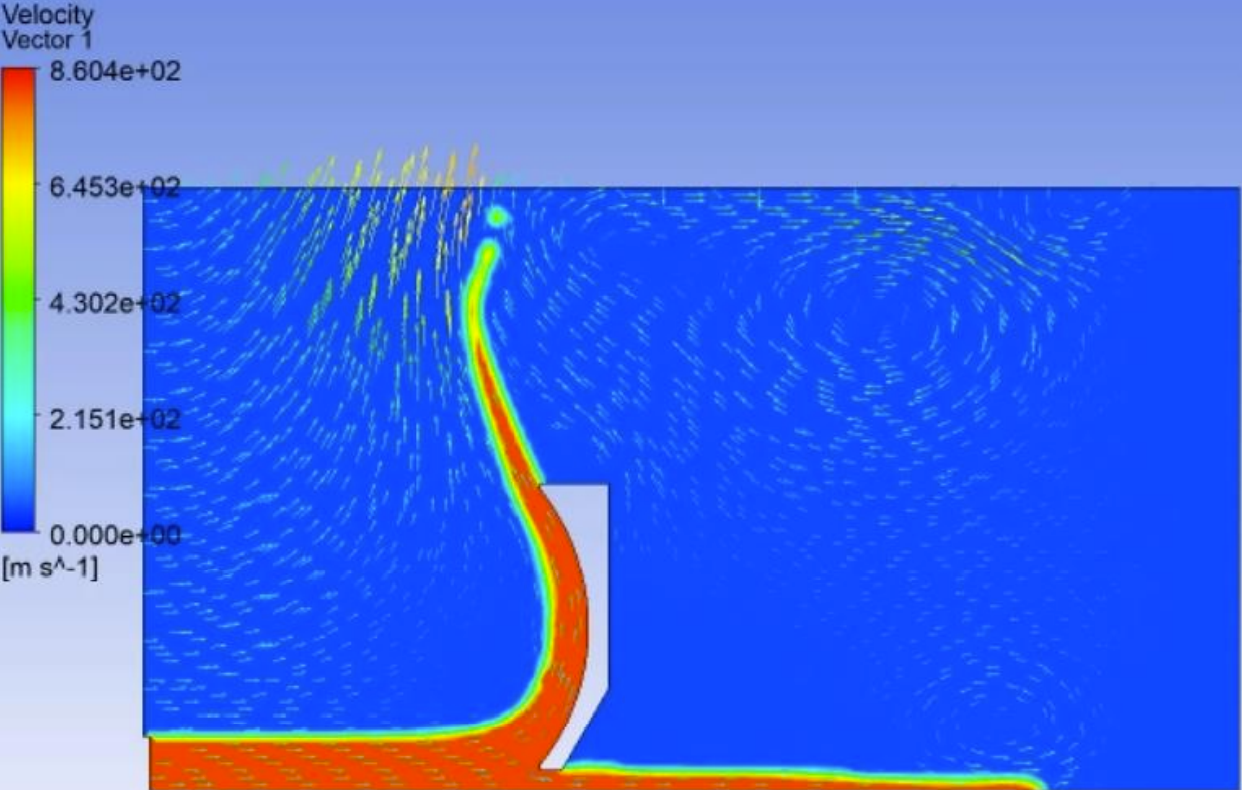
\includegraphics[width=\linewidth]{figures/fluid_sim2.png}
    \caption{Velocity Inlet = $250 m/s$, Time = $0.025sec$}
\end{figure}

The 7 measurements stored for each data sample in the simulation were:
\begin{itemize}
    \item The x-coordinate of the node, $x$
    \item The y-coordinate of the node, $y$
    \item The timestep, $t$
    \item The pressure (in atmospheres), $p$
    \item The u-velocity representing the x-component of the velocity field, $u$
    \item The v-velocity representing the y-component of the velocity field, $v$
    \item The water volume fraction or percentage of water from 0 to 1, $w.vf$
\end{itemize}

From now on, we will refer to data samples with the letter $x$, so for example $x^p$ is the pressure of the sample $x$ and $x_t^p$ is the pressure of the sample $x$ at a specific point in time $t$.

\subsection{Measuring Network Performance With The Mean Squared Error}
To measure the performance of our neural network we used a metric called \textbf{Mean Squared Error} which computes how erroneous our predictions were on average from the real values. The metric is defined in Equation \ref{eq:mse} below.
\begin{equation} \label{eq:mse}
    \frac{1}{n} \sum_{i=1}^{n}(y_{pred}-y_{true})^2
\end{equation}

where $y_{true}$ was the real value, $y_{pred}$ was our predicted value, and $n$ was the number of values or samples we were comparing.

For perfect predictions the value of $MSE = 0$. Therefore, the closer to 0 the better a model is performing.

\subsection{Proposed Network Architecture}
The proposed two-branch neural network took a range of time of measurements as input called the ``lookback'' and outputted the velocity components $u$ and $v$ that were predicted for the same position in space for the next timestep. The LSTM branch incorporated knowledge about the sequence and the Physics-Informed branch incorporated knowledge about the Partial Differential Equations (PDEs) describing in-compressible 2D discrete Navier-Stokes fluid flows. The architecture looked as follows:

% TODO: Re-render in higher quality as we have the original draw.io files
\begin{figure}[H] \label{fig:physics_lstm_architecture} \centering
    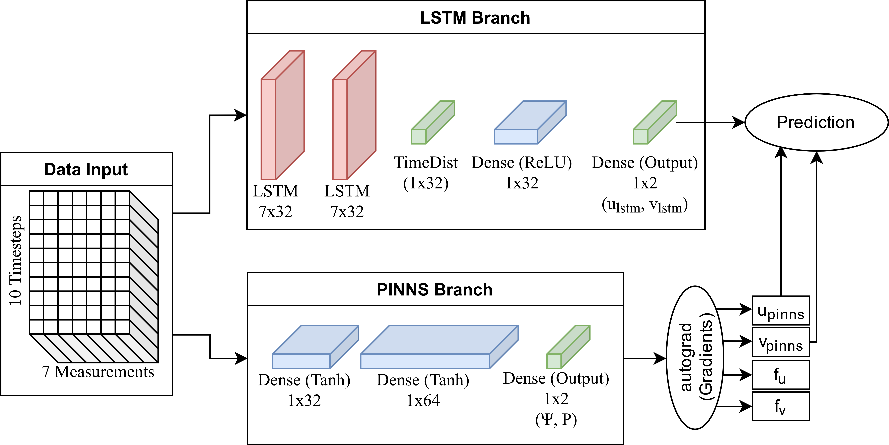
\includegraphics[width=\linewidth]{figures/physics_lstm_architecture.png}
    \caption{Physics-Informed LSTM Architecture showing both the LSTM and Physics-Informed branches and their connection to the final output prediction.}
\end{figure}

\subsubsection{LSTM Branch}
The LSTM branch had two stacked bi-directional LSTM layers with 32 activations each, followed by a Time Distributed layer that used a fully connected layer of 32 activations with a linear activation function. The Time Distributed layer applied the same weights to the previous LSTM outputs one timestep at a time. The LSTM layers were followed by a fully connected layer with 32 activations using the ReLU \cite{ReLU} non-linear activation function which was then followed by a fully connected output layer. The output layer consisted of two outputs, the x-component of the velocity field called u which was represented as $u_{lstm}$ and the y-component of the velocity field called v which was represented as $v_{lstm}$. The LSTM layers were connected to the fully connected part of the network by concatenating the two directional hidden states outputted by the last LSTM layer.

\subsubsection{Physics-Informed Branch}
As described in \cite{PINNS}, the general 2D Navier-Stokes equations:

\begin{equation} \label{eq:navier_stokes}
\begin{split}
    u_t + p_x + \lambda_1 (uu_x + vu_y) - \lambda_2 (u_{xx} + u_{yy}) &= 0 \\
    v_t + p_y + \lambda_1 (uv_x + vv_y) - \lambda_2 (v_{xx} + v_{yy}) &= 0 \\
    u_x + v_y &= 0
\end{split}
\end{equation}

We assumed that for some latent function $\psi(x, y, t)$

\begin{equation}
\begin{split}
    u &= \psi_y \\
    v &= -\psi_x
\end{split}
\end{equation}

Then we approximated $\psi(x, y, t)$ using a dense neural network $f$ with three inputs $(x, y, t)$, two outputs ($u, v$), and two learnable parameters $(\lambda_1, \lambda_2)$.

\begin{equation}
\begin{split}
    f_u(x,y,t) &:= u_t + p_x + \lambda_1 (uu_x + vu_y) - \lambda_2 (u_{xx} + u_{yy}) \\
    f_v(x,y,t) &:= v_t + p_y + \lambda_1 (uv_x + vv_y) - \lambda_2 (v_{xx} + v_{yy})
\end{split}
\end{equation}

The combined physics loss we needed to minimize was then computed from the following four losses:
\begin{equation}
\begin{split}
    MSE_u &= \frac{1}{n} \sum_{i=1}^{n}(\psi_y - u^i)^2 \\
    MSE_v &= \frac{1}{n} \sum_{i=1}^{n}(-\psi_x - v^i)^2 \\
    MSE_{f_u} &= \frac{1}{n} \sum_{i=1}^{n}(f_u(x^i,y^i,t^i))^2 \\
    MSE_{f_v} &= \frac{1}{n} \sum_{i=1}^{n}(f_v(x^i,y^i,t^i))^2
\end{split}
\end{equation}

Such that the total loss was:

\begin{equation}
    MSE_{total} = MSE_u + MSE_v + MSE_{f_u} + MSE_{f_v}
\end{equation}

The architecture consisted of a simple dense network with 3 layers. The first layer had 32 activations and used the hyperbolic tangent non-linear activation function (tanh), followed by another fully connected layer with 64 activations using tanh once again, followed by the output layer with two outputs. The automatic differentiation system included in PyTorch named \textbf{autograd} was used to compute the partial derivatives required for the computation of the final physics loss.

\subsubsection{Two-Branch Combined Model}
The two outputs of each branch were combined by using a weight $\alpha$ that was set between 0 and 1. For our experiments, $\alpha = 0.5$ (but in the future it could be set as a learnable parameter)

\begin{equation}
\begin{split}
    u_{pred} &= \alpha * u_{lstm} + (1 - \alpha) * u_{pinns} \\
    v_{pred} &= \alpha * v_{lstm} + (1 - \alpha) * v_{pinns}
\end{split}
\end{equation}

where $(u_{pred}, v_{pred})$ were the final predictions, ($u_{lstm}$, $v_{lstm}$) were the two outputs of the LSTM branch, and $(u_{pinns}, v_{pinns})$ were the two outputs of the Physics-Informed branch.


\subsection{Baseline Used To Compare Against Our Proposed Network}
The baseline used for this model was to simply assume that the velocities at the next timestep will be the same as those in the previous timestep for each data point.

\begin{equation} \label{eq:no_change_baseline}
\begin{split}
    prev_u &= x_{t}^{u} \\
    prev_v &= x_{t}^{v} \\
    y_{t+1}^{pred} &= (prev_u, prev_t)
\end{split}
\end{equation}

where $t$ was the current timestep, $x_t$ was the current data sample, $x_t^u$ was the u-velocity component of $x_t$, $y_t^v$ was the v-velocity component of $x_t$, and $y_{t+1}^{pred}$ was our predicted velocity.

\subsection{Experimental Results}
The following table summarizes the results of the experiments and provides the mean squared error for the velocity components \textbf{U} and \textbf{V} for each model along with the total training time after 200 epochs. The experiments were performed using an NVIDIA RTX 3090 and every epoch took around 27 seconds for non-informed LSTM models and 30 seconds for physics-informed LSTM models.

\begin{table}[h!] \centering
    \begin{tabular}{c|c|c|c}
        \textbf{Model} & \textbf{U} & \textbf{V} & \textbf{Time (min)} \\ \hline
        Baseline & 5.455 & 2.561 & 0.061 \\ \hline
        PINNS Only & 5709 & 12038 & 80 \\ \hline
        LSTM Only & 1.7811 & 8.6962 & 117 \\ \hline
        PINNS+LSTM & \textbf{0.4677} & \textbf{1.2794} & 142 \\ \hline
    \end{tabular}
    \caption{Comparison of the performance (MSE) of different models when using the 250m/s simulation for training and the 300m/s simulation for testing.}
    \label{tab:physics_lstm_results}
\end{table}

%LSTM ONLY TAKES 49sec for training epochs + 48 for validation except in 10_000 epoch one takes 1:28 + 1:23
% Physics-LSTM takes 1:11 + 1:03 -> 1:45 + 1:45
% PINNS takes 1:50 + 1:47

\subsection{Conclusion}
Our experimental results in Table \ref{tab:physics_lstm_results} show that the Physics-Informed LSTM outperforms the non-informed LSTM approach and leads us to our conclusion that informing the LSTM about the governing physics leads to better performance than just using LSTMs or PINNs by themselves.